\section{Módulo deportista}
En esta sección se describen los diferentes casos de uso asociados a este actor (ver figura \ref{fig:diagrama_cu_deportista}). En dicha figura se pueden observar los diferentes casos de uso asociados al deportista.

\begin{figure}[h!]
    \centering
    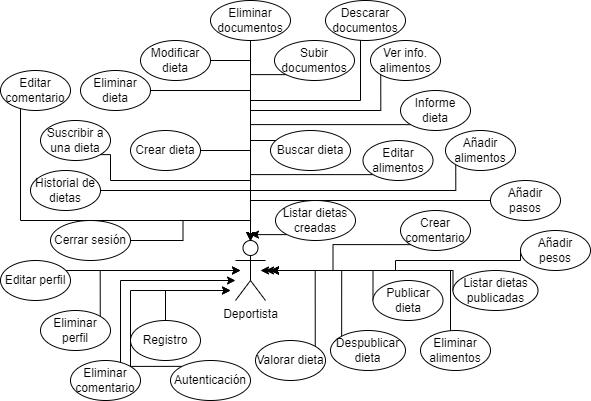
\includegraphics[width=0.75\textwidth]{Images/Capitulo4/cu-deportista.png}
    \caption{Diagrama de casos de uso asociado al actor \textit{Deportista}}
    \label{fig:diagrama_cu_deportista}
\end{figure}

\newpage % para bajar el 4.3 y que no quede entre tablas

%%%%%%%%%%%%%%%%%%%%%%%%
% TABLA 1
%%%%%%%%%%%%%%%%%%%%%%%%
\begin{table}[H]
\centering
\resizebox{\textwidth}{!}{%
\begin{tabular}{|l|l|}
\hline
\rowcolor[HTML]{8BC75F} 
\textbf{CU-01}         & \textbf{Registrar deportista}                                                                       \\ \hline
Descripción            & \begin{tabular}[c]{@{}l@{}}El deportista podrá registrarse en la aplicación para poder utilizar\\ las funciones básicas de la misma\end{tabular}                                                                         \\ \hline
Actor                  & Deportista                                                                                                                                                                                                            \\ \hline
Entrada                & Datos del deportista                                                                                                                                                                                                     \\ \hline
Salida                 & Mensaje de éxito o error                                                                                                                                                                                              \\ \hline
Origen                 & Página de registro                                                                                                                                                                                          \\ \hline
Precondición           & No existe un usuario con el mismo correo electrónico                                                                                                                                                                  \\ \hline
Postcondición si éxito & El deportista se registra correctamente                                                                                                                                                                                  \\ \hline
Postcondición si fallo & Se vuelven a pedir los datos para proceder nuevamente al registro                                                                                                                                                     \\ \hline
Flujo normal           & \begin{tabular}[c]{@{}l@{}}1. Se pulsa en el botón de registro\\ 2. Se introducen los datos requeridos\\ 3. Se validan los datos\\ 4. Se pulsa sobre el botón de registrar y se da de alta el deportista\end{tabular}                          \\ \hline
Flujo alternativo      & \begin{tabular}[c]{@{}l@{}}2. Se introducen de forma incorrecta los datos o lo hace\\ con los de otro usuario ya registrado\\ 3. Se muestra un mensaje de error y se vuelven a pedir los datos\end{tabular} \\ \hline

\end{tabular}%
}
\caption{Registrar deportista}
\end{table}


%%%%%%%%%%%%%%%%%%%%%%%%
% TABLA 2
%%%%%%%%%%%%%%%%%%%%%%%%
\begin{table}[H]
\centering
\resizebox{\textwidth}{!}{%
\begin{tabular}{|l|l|}
\hline
\rowcolor[HTML]{8BC75F} 
\textbf{CU-02}         & \textbf{Autenticar deportista}\\ \hline
Descripción            & El deportista puede iniciar sesión en la aplicación con sus credenciales                                                                                                                                               \\ \hline
Actor                  & Deportista                                                                                                                                                                                                          \\ \hline
Entrada                & Credenciales de la cuenta del deportista                                                                                                                                                                            \\ \hline
Salida                 & Mensaje de éxito o error                                                                                                                                                                                            \\ \hline
Origen                 & Página de inicio de sesión de la aplicación                                                                                                                                                                         \\ \hline
Precondición           & \begin{tabular}[c]{@{}l@{}}El deportista debe tener una cuenta creada con las credenciales\\ proporcionadas\end{tabular}                                                                                               \\ \hline
Postcondición si éxito & El deportista inicia sesión satisfactoriamente                                                                                                                                                                         \\ \hline
Postcondición si fallo & Se vuelven a pedir los datos nuevamente                                                                                                                                                                             \\ \hline
Flujo normal           & \begin{tabular}[c]{@{}l@{}}1. Se pulsa en el botón de iniciar sesión\\ 2. Se introducen las credenciales necesarias para la acción\\ 3. Se validan las credenciales y se inicia sesión\end{tabular} \\ \hline
Flujo alternativo      & \begin{tabular}[c]{@{}l@{}}2. Se introducen unas credenciales incorrectas\\ 3. Los datos no son validados y se muestra un mensaje de error\end{tabular}                                                   \\ \hline
\end{tabular}%
}
\caption{Autenticar deportista}
\end{table}


%%%%%%%%%%%%%%%%%%%%%%%%
% TABLA 3
%%%%%%%%%%%%%%%%%%%%%%%%
\begin{table}[H]
\centering
\resizebox{\textwidth}{!}{%
\begin{tabular}{|l|l|}
\hline
\rowcolor[HTML]{8BC75F} 
\textbf{CU-03}         & \textbf{Cerrar la sesión de un deportista}\\ \hline
Descripción            & El deportista cierra su sesión activa en la aplicación                                                                                                                     \\ \hline
Actor                  & Deportista                                                                                                                                                                 \\ \hline
Entrada                & NA                                                                                                                                                                         \\ \hline
Salida                 & NA                                                                                                                                                                         \\ \hline
Origen                 & Desplegable de opciones del perfil del deportista                                                                                                                             \\ \hline
Precondición           & El deportista debe de haber iniciado sesión                                                                                                                                   \\ \hline
Postcondición si éxito & Se cierra la sesión activa del deportista                                                                                                                                  \\ \hline
Postcondición si fallo & La sesión del deportista no se cierra debido a un error                                                                                                                                  \\ \hline
Flujo normal           & \begin{tabular}[c]{@{}l@{}}1. Se accede desde el menú principal al perfil del deportista \\ 2. Se pulsa sobre las opciones del perfil\\ 3. Se selecciona la opción de cerrar sesión\end{tabular} \\ \hline
Flujo alternativo      & NA                                                                                                                                                                         \\ \hline

\end{tabular}%
}
\caption{Cerrar la sesión de un deportista}
\end{table}

%%%%%%%%%%%%%%%%%%%%%%%%
% TABLA 4
%%%%%%%%%%%%%%%%%%%%%%%%
\begin{table}[H]
\centering
\resizebox{\textwidth}{!}{%
\begin{tabular}{|l|l|}
\hline
\rowcolor[HTML]{8BC75F} 
\textbf{CU-04}         & \textbf{Modificar datos de un deportista}\\ \hline
Descripción            & El deportista modifica los datos de su cuenta                                                                                                                                                                                                                                         \\ \hline
Actor                  & Deportista                                                                                                                                                                                                                                                                            \\ \hline
Entrada                & Los datos modificados que se van a actualizar                                                                                                                                                                                                                                         \\ \hline
Salida                 & Mensaje de éxito o error                                                                                                                                                                                                                                                              \\ \hline
Origen                 & Vista de modificar datos del deportista                                                                                                                                                                                                                                               \\ \hline
Precondición           & El deportista debe de haber iniciado sesión                                                                                                                                                                                                                                              \\ \hline
Postcondición si éxito & Los datos del deportista son actualizados en la aplicación                                                                                                                                                                                                                               \\ \hline
Postcondición si fallo & \begin{tabular}[c]{@{}l@{}}Se vuelven a pedir los datos nuevamente tras haber mostrado un\\ mensaje de error\end{tabular}                                                                                                                                                             \\ \hline
Flujo normal           & \begin{tabular}[c]{@{}l@{}}1. Se accede desde el menú principal al perfil del deportista \\ 2. Se pulsa sobre las opciones del perfil\\ 3. Se selecciona la opción de editar perfil\\ 4. Se introducen los nuevos datos que se quieran modificar\\ 5. Se validan y actualizan en la aplicación\end{tabular} \\ \hline
Flujo alternativo      & \begin{tabular}[c]{@{}l@{}}4. El deportista introduce algún dato erróneo o vacío y se muestra\\ un mensaje de error\end{tabular}                                                                                                                                                      \\ \hline
\end{tabular}%
}
\caption{Modificar datos de un deportista}
\end{table}



%%%%%%%%%%%%%%%%%%%%%%%%
% TABLA 5
%%%%%%%%%%%%%%%%%%%%%%%%
\begin{table}[H]
\centering
\resizebox{\textwidth}{!}{%
\begin{tabular}{|l|l|}
\hline
\rowcolor[HTML]{8BC75F} 
\textbf{CU-05}         & \textbf{Eliminar perfil de un deportista}\\ \hline
Descripción            & Se elimina la cuenta del deportista                                                                                                                                                                                                        \\ \hline
Actor                  & Deportista                                                                                                                                                                                                                                 \\ \hline
Entrada                & Confirmación del deportista                                                                                                                                                                                                                   \\ \hline
Salida                 & Mensaje de éxito o error si se ha borrado el perfil satisfactoriamente                                                                                                                                                                     \\ \hline
Origen                 & Vista del perfil del deportista                                                                                                                                                                                                            \\ \hline
Precondición           & El deportista debe tener una cuenta activa y debe de haber iniciado sesión                                                                                                                                                                    \\ \hline
Postcondición si éxito & Se elimina la cuenta del deportista del sistema                                                                                                                                                                                               \\ \hline
Postcondición si fallo & La cuenta del deportista no se ve alterada                                                                                                                                                                                                 \\ \hline
Flujo normal           & \begin{tabular}[c]{@{}l@{}}1. Se accede desde el menú principal al perfil del deportista\\ 2. Se pulsa sobre las opciones del perfil\\ 3. Se selecciona la opción de eliminar cuenta\\ 4. Se elimina la cuenta del deportista tras la confirmación\end{tabular} \\ \hline
Flujo alternativo      & 4. El deportista deniega la confirmación de borrar cuenta y no sucede nada                                                                                                                                                                 \\ \hline

\end{tabular}%
}
\caption{Eliminar perfil de un deportista}
\end{table}


%%%%%%%%%%%%%%%%%%%%%%%%
% TABLA 6
%%%%%%%%%%%%%%%%%%%%%%%%
\begin{table}[H]
\centering
\resizebox{\textwidth}{!}{%
\begin{tabular}{|l|l|}
\hline
\rowcolor[HTML]{8BC75F} 
\textbf{CU-06}         & \textbf{Creación de una dieta}\\ \hline
Descripción            & El deportista crea una dieta en el sistema                                                                                                                                                                                                                                                                                              \\ \hline
Actor                  & Deportista                                                                                                                                                                                                                                                                                                                              \\ \hline
Entrada                & Datos de la dieta                                                                                                                                                                                                                                                                                                                       \\ \hline
Salida                 & Mensaje de éxito o error                                                                                                                                                                                                                                                                                                                \\ \hline
Origen                 & Vista de crear una dieta                                                                                                                                                                                                                                                                                                                \\ \hline
Precondición           & El deportista debe tener una cuenta activa y debe de haber iniciado sesión                                                                                                                                                                                                                                                                 \\ \hline
Postcondición si éxito & Se crea la dieta para el deportista                                                                                                                                                                                                                                                                                                     \\ \hline
Postcondición si fallo & Mensaje de error y se vuelven a pedir los datos                                                                                                                                                                                                                                                                                         \\ \hline
Flujo normal           & \begin{tabular}[c]{@{}l@{}}1. Desde el menú principal se  pulsa sobre las dietas creadas por\\ el deportista\\ 2. Se pulsa sobre el botón inferior en la zona derecha con el símbolo ``$+$``\\ 3. Se introducen los datos requeridos para crear la dieta\\ 4. Se pulsa sobre el botón de guardar y se crea la dieta\end{tabular} \\ \hline
Flujo alternativo      & \begin{tabular}[c]{@{}l@{}}3. El deportista no rellena algún campo requerido\\ 4. Se pulsa sobre el botón guardar y aparece un mensaje de error\end{tabular}                                                                                                                                                                            \\ \hline
\end{tabular}%
}
\caption{El deportista crea una dieta}
\end{table}

%%%%%%%%%%%%%%%%%%%%%%%%
% TABLA 7
%%%%%%%%%%%%%%%%%%%%%%%%
\begin{table}[H]
\centering
\resizebox{\textwidth}{!}{%
\begin{tabular}{|l|l|}
\hline
\rowcolor[HTML]{8BC75F} 
\textbf{CU-07}         & \textbf{Subir documentos a una dieta}\\ \hline
Descripción            & El deportista sube documentos a una de sus dietas creadas                                                                                                                                                                                                                                                                            \\ \hline
Actor                  & Deportista                                                                                                                                                                                                                                                                                                                           \\ \hline
Entrada                & Documento seleccionado de los archivos del smartphone                                                                                                                                                                                                                                                                                \\ \hline
Salida                 & Mensaje de éxito o error                                                                                                                                                                                                                                                                                                             \\ \hline
Origen                 & Vista de editar dieta creada por el deportista                                                                                                                                                                                                                                                                                       \\ \hline
Precondición           & La dieta debe pertenecer al deportista                                                                                                                                                                                                                                                                                               \\ \hline
Postcondición si éxito & El documento es asociado a la dieta                                                                                                                                                                                                                                                                                                  \\ \hline
Postcondición si fallo & El documento no se sube y por lo tanto el estado de la dieta es alterado                                                                                                                                                                                                                                                             \\ \hline
Flujo normal           & \begin{tabular}[c]{@{}l@{}}1. El deportista pulsa sobre el botón de ver todas las dietas creadas\\ 2. Se accede a la dieta a la que se quiera subir el documento\\ 3. Se pulsa sobre el botón de editar dieta\\ 4. El deportista pulsa sobre el botón de subir documento\\ 5. Se selecciona un documento del smartphone\end{tabular} \\ \hline
Flujo alternativo      & \begin{tabular}[c]{@{}l@{}}5. El deportista no selecciona ningún documento y la operación de\\ subida se cancela\end{tabular}                                                                                                                                                                                                        \\ \hline

\end{tabular}%
}
\caption{Subir documentos a una dieta}
\end{table}


%%%%%%%%%%%%%%%%%%%%%%%%
% TABLA 7
%%%%%%%%%%%%%%%%%%%%%%%%
\begin{table}[H]
\centering
\resizebox{\textwidth}{!}{%
\begin{tabular}{|l|l|}
\hline
\rowcolor[HTML]{8BC75F} 
\textbf{CU-08}         & \textbf{Eliminar documentos de una dieta}\\ \hline
Descripción            & El deportista elimina documentos a una de sus dietas creadas                                                                                                                                                                                                                         \\ \hline
Actor                  & Deportista                                                                                                                                                                                                                                                                           \\ \hline
Entrada                & Identificador del documento que se quiere eliminar                                                                                                                                                                                                                                   \\ \hline
Salida                 & Mensaje de éxito o error                                                                                                                                                                                                                                                             \\ \hline
Origen                 & Vista de edición de la dieta                                                                                                                                                                                                                                                         \\ \hline
Precondición           & El documento debe existir y estar asociado a la dieta                                                                                                                                                                                                                                \\ \hline
Postcondición si éxito & El documento es eliminado de la dieta                                                                                                                                                                                                                                                \\ \hline
Postcondición si fallo & El documento no se elimina y por lo tanto sigue asociado a la dieta                                                                                                                                                                                                                  \\ \hline
Flujo normal           & \begin{tabular}[c]{@{}l@{}}1. El deportista pulsa sobre el botón de ver todas las dietas creadas\\ 2. Se accede a la dieta de la que se quiera eliminar un documento\\ 3. Se pulsa sobre el botón de editar la dieta\\ 4. Se pulsa sobre la ``{\color{red}$X$}`` situada junto al documento\end{tabular} \\ \hline
Flujo alternativo      & NA                                                                                                                                                                                                                                                                                   \\ \hline

\end{tabular}%
}
\caption{Eliminar documentos de una dieta}
\end{table}


%%%%%%%%%%%%%%%%%%%%%%%%
% TABLA 7
%%%%%%%%%%%%%%%%%%%%%%%%
\begin{table}[H]
\centering
\resizebox{\textwidth}{!}{%
\begin{tabular}{|l|l|}
\hline
\rowcolor[HTML]{8BC75F} 
\textbf{CU-09}         & \textbf{Descargar documentos de una dieta}\\ \hline
Descripción            & El deportista descarga un documento de una dieta                                                                                                                                                                                                            \\ \hline
Actor                  & Deportista                                                                                                                                                                                                                                                  \\ \hline
Entrada                & Identificador del documento que se quiere descargar                                                                                                                                                                                                         \\ \hline
Salida                 & NA                                                                                                                                                                                                                                                          \\ \hline
Origen                 & Vista detallada de una dieta                                                                                                                                                                                                                                \\ \hline
Precondición           & El documento debe existir y estar asociado a la dieta                                                                                                                                                                                                       \\ \hline
Postcondición si éxito & El documento es descargado en el smartphone del usuario                                                                                                                                                                                                     \\ \hline
Postcondición si fallo & El documento no se descarga debido a un error                                                                                                                                                                                                               \\ \hline
Flujo normal           & \begin{tabular}[c]{@{}l@{}}1. El deportista pulsa sobre el botón de ver todas las dietas publicadas\\ 2. Se accede a la dieta de la que se quiera descargar el documento\\ 3. Se pulsa sobre el icono de la flecha para descargar el documento\end{tabular} \\ \hline
Flujo alternativo      & NA                                                                                                                                                                                                                                                          \\ \hline

\end{tabular}%
}
\caption{Descargar documentos de una dieta}
\end{table}


%%%%%%%%%%%%%%%%%%%%%%%%
% TABLA 8
%%%%%%%%%%%%%%%%%%%%%%%%
\begin{table}[H]
\centering
\resizebox{\textwidth}{!}{%
\begin{tabular}{|l|l|}
\hline
\rowcolor[HTML]{8BC75F} 
\textbf{CU-10}         & \textbf{Suscribirse a una dieta}\\ \hline
Descripción            & El deportista se suscribe a una de las dietas publicadas en el sistema                                                                                                                                                                                      \\ \hline
Actor                  & Deportista                                                                                                                                                                                                                                                  \\ \hline
Entrada                & Confirmación del deportista                                                                                                                                                                                                                                    \\ \hline
Salida                 & Mensaje de éxito o error                                                                                                                                                                                                                                    \\ \hline
Origen                 & Vista de todas las dietas publicadas del sistema                                                                                                                                                                                                            \\ \hline
Precondición           & La dieta a la que se quiera suscribir debe estar publicada                                                                                                                                                                                                  \\ \hline
Postcondición si éxito & El deportista se suscribe a la dieta elegida                                                                                                                                                                                                                \\ \hline
Postcondición si fallo & NA                                                                                                                                                                                                                                                          \\ \hline
Flujo normal           & \begin{tabular}[c]{@{}l@{}}1. Desde el menú principal se pulsa sobre el botón de dietas publicadas\\ 2. Se accede a ver la dieta que desea seguir\\ 3. Se pulsa sobre el icono ``$\star$`` para empezar a seguir la dieta\end{tabular} \\ \hline
Flujo alternativo      & \begin{tabular}[c]{@{}l@{}}4. Si el deportista ya sigue una dieta se muestra un aviso\\ 5. Se confirma que quiere seguir la nueva dieta y se\\ suscribe a dicha dieta\end{tabular}                                                               \\ \hline
\end{tabular}%
}
\caption{Suscribirse a una dieta}
\end{table}


%%%%%%%%%%%%%%%%%%%%%%%%
% TABLA 8
%%%%%%%%%%%%%%%%%%%%%%%%
\begin{table}[H]
\centering
\resizebox{\textwidth}{!}{%
\begin{tabular}{|l|l|}
\hline
\rowcolor[HTML]{8BC75F} 
\textbf{CU-11}         & \textbf{Modificar una dieta creada por el deportista}\\ \hline
Descripción            & \begin{tabular}[c]{@{}l@{}}El deportista modifica los diferentes campos de una de sus dietas\\ creadas o añade alimentos a la misma\end{tabular}                                                                                                                                                                                                                                        \\ \hline
Actor                  & Deportista                                                                                                                                                                                                                                                                                                                                                                              \\ \hline
Entrada                & Datos nuevos de la dieta                                                                                                                                                                                                                                                                                                                                                                \\ \hline
Salida                 & Mensaje de éxito o error                                                                                                                                                                                                                                                                                                                                                                \\ \hline
Origen                 & Vista de las dietas creadas por el deportista                                                                                                                                                                                                                                                                                                                                           \\ \hline
Precondición           & La dieta que se quiere editar debe existir y pertenecer al deportista                                                                                                                                                                                                                                                                                                                   \\ \hline
Postcondición si éxito & Los datos de la dieta se modifican satisfactoriamente                                                                                                                                                                                                                                                                                                                                   \\ \hline
Postcondición si fallo & Aviso del error sucedido                                                                                                                                                                                                                                                                                                                                                                \\ \hline
Flujo normal           & \begin{tabular}[c]{@{}l@{}}1. Desde el menú principal se pulsa sobre las dietas creadas\\ 2. Se accede a ver la dieta que se quiera editar\\ 3. Se pulsa sobre el botón de editar la dieta\\ 4. Se actualizna los campos de la dieta o se añaden, eliminan\\ y/o modifican alimentos de la misma\\ 5. Se pulsa sobre el botón de guardar para actualizar la dieta\end{tabular} \\ \hline
Flujo alternativo      & \begin{tabular}[c]{@{}l@{}}4. El deportista introduce de forma incorrecta alguno de los campos\\ de la dieta\\ 5. Se muestra un mensaje de error mostrando el fallo ocurrido\end{tabular}                                                                                                                                                                                               \\ \hline
\end{tabular}%
}
\caption{Modificar una dieta creada por el deportista}
\end{table}


%%%%%%%%%%%%%%%%%%%%%%%%
% TABLA 9
%%%%%%%%%%%%%%%%%%%%%%%%
\begin{table}[H]
\centering
\resizebox{\textwidth}{!}{%
\begin{tabular}{|l|l|}
\hline
\rowcolor[HTML]{8BC75F} 
\textbf{CU-12}         & \textbf{Ver historial de dietas seguidas}\\ \hline
Descripción            & El deportista puede ver el histórico de dietas seguidas anteriormente                                                                                                                                                                                                \\ \hline
Actor                  & Deportista                                                                                                                                                                                                                                                           \\ \hline
Entrada                & NA                                                                                                                                                                                                                                                                   \\ \hline
Salida                 & Listado de todas las dietas que ha seguido el deportista                                                                                                                                                                                                             \\ \hline
Origen                 & Vista del histórico de dietas                                                                                                                                                                                                                                        \\ \hline
Precondición           & El deportista debe existir en el sistema                                                                                                                                                                                                                             \\ \hline
Postcondición si éxito & \begin{tabular}[c]{@{}l@{}}Se muestra una tabla con información de las dietas que ha seguido\\ el deportista\end{tabular}                                                                                                                                            \\ \hline
Postcondición si fallo & NA                                                                                                                                                                                                                                                                   \\ \hline
Flujo normal           & \begin{tabular}[c]{@{}l@{}}1. Desde el menú principal se pulsa sobre el botón de ver perfil\\ 2. Se pulsa sobre las opciones del perfil\\ 3. Se pulsa sobre ver el historial de dietas\\ 4. Se muestran todas las dietas que seguido el deportista\end{tabular} \\ \hline
Flujo alternativo      & NA                                                                                                                                                                                                                                                                   \\ \hline
\end{tabular}%
}
\caption{Ver historial de dietas seguidas}
\end{table}


%%%%%%%%%%%%%%%%%%%%%%%%
% TABLA 10
%%%%%%%%%%%%%%%%%%%%%%%%
\begin{table}[H]
\centering
\resizebox{\textwidth}{!}{%
\begin{tabular}{|l|l|}
\hline
\rowcolor[HTML]{8BC75F} 
\textbf{CU-13}         & \textbf{Eliminar una dieta creada por del deportista}\\ \hline
Descripción            & El deportista elimina una de las dietas que ha creado                                                                                                                                                                                                                                                                          \\ \hline
Actor                  & Deportista                                                                                                                                                                                                                                                                                                                     \\ \hline
Entrada                & Confirmación del deportista                                                                                                                                                                                                                                                                                                       \\ \hline
Salida                 & Mensaje de éxito o error                                                                                                                                                                                                                                                                                                       \\ \hline
Origen                 & Vista de ver detalles de la dieta                                                                                                                                                                                                                                                                                              \\ \hline
Precondición           & La dieta que se quiera eliminar debe existir                                                                                                                                                                                                                                                                                   \\ \hline
Postcondición si éxito & Mensaje de éxito y eliminación de la dieta                                                                                                                                                                                                                                                                                     \\ \hline
Postcondición si fallo & Mensaje de error indicando el fallo                                                                                                                                                                                                                                                                                            \\ \hline
Flujo normal           & \begin{tabular}[c]{@{}l@{}}1. Desde la página principal se pulsa sobre el botón de dietas creadas\\ 2. Se pulsa sobre ver dieta para acceder a la vista en detalle de la misma\\ 3. Se pulsa sobre el botón de eliminar dieta\\ 4. Se muestra y acepta un mensaje de confirmación para eliminarla\end{tabular} \\ \hline
Flujo alternativo      & \begin{tabular}[c]{@{}l@{}}4. El deportista deniega la confirmación de eliminar la dieta y no se\\ realiza ninguna acción sobre la misma\end{tabular}                                                                                                                                                                          \\ \hline
\end{tabular}%
}
\caption{Eliminar una dieta creada por del deportista}
\end{table}


%%%%%%%%%%%%%%%%%%%%%%%%
% TABLA 11
%%%%%%%%%%%%%%%%%%%%%%%%
\begin{table}[H]
\centering
\resizebox{\textwidth}{!}{%
\begin{tabular}{|l|l|}
\hline
\rowcolor[HTML]{8BC75F} 
\textbf{CU-14}         & \textbf{Listar dietas creadas por del deportista}\\ \hline
Descripción            & Se muestran todas las dietas que el deportista ha creado                                                                                                                 \\ \hline
Actor                  & Deportista                                                                                                                                                               \\ \hline
Entrada                & Identificador del deportista                                                                                                                                                \\ \hline
Salida                 & Todas las dietas del deportista                                                                                                                                             \\ \hline
Origen                 & Vista de ver todas las dietas                                                                                                                                            \\ \hline
Precondición           & El deportista debe tener una cuenta activa en el sistema                                                                                                                    \\ \hline
Postcondición si éxito & Se muestran todas las dietas que el deportista ha creado                                                                                                                    \\ \hline
Postcondición si fallo & NA                                                                                                                                                                       \\ \hline
Flujo normal           & \begin{tabular}[c]{@{}l@{}}1. Desde la página principal se pulsa sobre el botón de dietas creadas\\ 2. Todas las dietas creadas por el deportista son listadas\end{tabular} \\ \hline
Flujo alternativo      & NA                                                                                                                                                                       \\ \hline

\end{tabular}%
}
\caption{Listar dietas creadas por del deportista}
\end{table}


%%%%%%%%%%%%%%%%%%%%%%%%
% TABLA 12
%%%%%%%%%%%%%%%%%%%%%%%%
\begin{table}[H]
\centering
\resizebox{\textwidth}{!}{%
\begin{tabular}{|l|l|}
\hline
\rowcolor[HTML]{8BC75F} 
\textbf{CU-15}         & \textbf{Ver todas las dietas publicadas del sistema}\\ \hline
Descripción            & Se muestran todas las dietas publicadas del sistema                                                                                                                           \\ \hline
Actor                  & Deportista                                                                                                                                                                    \\ \hline
Entrada                & NA                                                                                                                                                                            \\ \hline
Salida                 & Todas las dietas publicadas que hay en el sistema                                                                                                                             \\ \hline
Origen                 & Vista de todas las dietas publicadas                                                                                                                                          \\ \hline
Precondición           & Tiene que haber dietas que los usuarios hayan publicado                                                                                                                       \\ \hline
Postcondición si éxito & Se muestran todas las dietas publicadas en formato tabla                                                                                                                      \\ \hline
Postcondición si fallo & NA                                                                                                                                                                            \\ \hline
Flujo normal           & \begin{tabular}[c]{@{}l@{}}1. Desde la página principal se pulsa sobre el botón de dietas publicadas\\ 2. Todas las dietas publicadas en el sistema son listadas\end{tabular} \\ \hline
Flujo alternativo      & NA                                                                                                                                                                            \\ \hline

\end{tabular}%
}
\caption{Ver todas las dietas publicadas del sistema}
\end{table}


%%%%%%%%%%%%%%%%%%%%%%%%
% TABLA 13
%%%%%%%%%%%%%%%%%%%%%%%%
\begin{table}[H]
\centering
\resizebox{\textwidth}{!}{%
\begin{tabular}{|l|l|}
\hline
\rowcolor[HTML]{8BC75F} 
\textbf{CU-16}         & \textbf{Buscar dietas}\\ \hline
Descripción            & El deportista busca una dieta entre todas las dietas publicadas                                                                                                                                                                                                     \\ \hline
Actor                  & Deportista                                                                                                                                                                                                                                                          \\ \hline
Entrada                & Texto introducido por el deportista sobre el que buscar dietas                                                                                                                                                                                                         \\ \hline
Salida                 & \begin{tabular}[c]{@{}l@{}}Todas las dietas publicadas cuyos títulos coinciden de cierta forma\\ con el texto introducido\end{tabular}                                                                                                                              \\ \hline
Origen                 & Vista de todas las dietas publicadas                                                                                                                                                                                                                                \\ \hline
Precondición           & Tiene que haber dietas publicadas en el sistema                                                                                                                                                                                                                     \\ \hline
Postcondición si éxito & \begin{tabular}[c]{@{}l@{}}Se muestran todas las dietas publicadas con un título similar al texto\\ introducido\end{tabular}                                                                                                                                        \\ \hline
Postcondición si fallo & No se muestra ninguna dieta en la tabla de la correspondiente vista                                                                                                                                                                                                 \\ \hline
Flujo normal           & \begin{tabular}[c]{@{}l@{}}1. Desde la página principal se pulsa sobre el botón de dietas publicadas\\ 2. Se escribe el texto deseado sobre la barra superior de búsqueda\\ 3. Se listan todas las dietas cuyos títulos coinciden con el texto buscado\end{tabular} \\ \hline
Flujo alternativo      & \begin{tabular}[c]{@{}l@{}}3. No hay dietas que coincidan con el texto de la búsqueda y por lo tanto\\ ninguna dieta es listada\end{tabular}                                                                                                                        \\ \hline

\end{tabular}%
}
\caption{Buscar dietas}
\end{table}


%%%%%%%%%%%%%%%%%%%%%%%%
% TABLA 14
%%%%%%%%%%%%%%%%%%%%%%%%
\begin{table}[H]
\centering
\resizebox{\textwidth}{!}{%
\begin{tabular}{|l|l|}
\hline
\rowcolor[HTML]{8BC75F} 
\textbf{CU-17}         & \textbf{Publicar una dieta creada por el deportista}\\ \hline
Descripción            & El deportista publica una de sus dietas creadas                                                                                                                                                                                                                                                     \\ \hline
Actor                  & Deportista                                                                                                                                                                                                                                                                                          \\ \hline
Entrada                & Identificador de la dieta que se quiere publicar                                                                                                                                                                                                                                                    \\ \hline
Salida                 & Mensaje de éxito o fallo si la dieta se ha publicado correctamente o no                                                                                                                                                                                                                             \\ \hline
Origen                 & Vista de ver la dieta                                                                                                                                                                                                                                                                               \\ \hline
Precondición           & La dieta debe existir y no debe estar publicada                                                                                                                                                                                                                                                  \\ \hline
Postcondición si éxito & Mensaje informando de que la dieta ha sido publicada correctamente                                                                                                                                                                                                                                  \\ \hline
Postcondición si fallo & Mensaje informando del error que se ha producido                                                                                                                                                                                                                                                    \\ \hline
Flujo normal           & \begin{tabular}[c]{@{}l@{}}1. Desde la página principal se pulsa sobre el botón de dietas creadas\\ 2. Se accede a ver la dieta que el deportista quiera publicar\\ 3. Se pulsa sobre el botón de publicar dieta\\ 4. Se muestra un mensaje informativo de que la dieta ha sido publicada\end{tabular} \\ \hline
Flujo alternativo      & \begin{tabular}[c]{@{}l@{}}3. Sucede algún error al momento de publicar la dieta se muestra un\\ mensaje y no se produce ninguna acción sobre la dieta\end{tabular}                                                                                                                                 \\ \hline

\end{tabular}%
}
\caption{Publicar una dieta creada por el deportista}
\end{table}


%%%%%%%%%%%%%%%%%%%%%%%%
% TABLA 15
%%%%%%%%%%%%%%%%%%%%%%%%
\begin{table}[H]
\centering
\resizebox{\textwidth}{!}{%
\begin{tabular}{|l|l|}
\hline
\rowcolor[HTML]{8BC75F} 
\textbf{CU-18}         & \textbf{Despublicar una dieta creada por el deportista}\\ \hline
Descripción            & El deportista despublica una de sus dietas creadas                                                                                                                                                                                                                                                           \\ \hline
Actor                  & Deportista                                                                                                                                                                                                                                                                                                   \\ \hline
Entrada                & Identificador de la dieta que se quiere despublicar                                                                                                                                                                                                                                                          \\ \hline
Salida                 & Mensaje de éxito o fallo si la dieta se ha despublicado correctamente o no                                                                                                                                                                                                                                   \\ \hline
Origen                 & Vista de ver la dieta                                                                                                                                                                                                                                                                                        \\ \hline
Precondición           & La dieta debe existir y debe estar publicada                                                                                                                                                                                                                                                                 \\ \hline
Postcondición si éxito & Mensaje informando de que la dieta ha sido despublicada correctamente                                                                                                                                                                                                                                        \\ \hline
Postcondición si fallo & Mensaje informando del error que se ha producido                                                                                                                                                                                                                                                             \\ \hline
Flujo normal           & \begin{tabular}[c]{@{}l@{}}1. Desde la página principal se pulsa sobre el botón de dietas creadas\\ 2. Se accede a ver la dieta que el deportista quiera despublicar\\ 3. Se pulsa sobre el botón de despublicar dieta\\ 4. Se muestra un mensaje informativo de que la dieta ha sido despublicada\end{tabular} \\ \hline
Flujo alternativo      & \begin{tabular}[c]{@{}l@{}}3. Sucede algún error al momento de despublicar la dieta se muestra un\\ mensaje y no se produce ninguna acción sobre la dieta\end{tabular}                                                                                                                                       \\ \hline
\end{tabular}%
}
\caption{Despublicar una dieta creada por el deportista}
\end{table}



%%%%%%%%%%%%%%%%%%%%%%%%
% TABLA 15
%%%%%%%%%%%%%%%%%%%%%%%%
\begin{table}[H]
\centering
\resizebox{\textwidth}{!}{%
\begin{tabular}{|l|l|}
\hline
\rowcolor[HTML]{8BC75F} 
\textbf{CU-19}         & \textbf{Añadir alimentos a una dieta}\\ \hline
Descripción            & El deportista añade alimentos a una de sus dietas creadas                                                                                                                                                                                                                                                                                                                                                                                                                                                        \\ \hline
Actor                  & Deportista                                                                                                                                                                                                                                                                                                                                                                                                                                                                                                       \\ \hline
Entrada                & Información del alimento que se quiere añadir                                                                                                                                                                                                                                                                                                                                                                                                                                                                    \\ \hline
Salida                 & Mensaje de éxito o error                                                                                                                                                                                                                                                                                                                                                                                                                                                                                         \\ \hline
Origen                 & Vista de editar dieta creada por el deportista                                                                                                                                                                                                                                                                                                                                                                                                                                                                   \\ \hline
Precondición           & La dieta debe pertenecer al deportista                                                                                                                                                                                                                                                                                                                                                                                                                                                                           \\ \hline
Postcondición si éxito & El alimento es añadido a la dieta                                                                                                                                                                                                                                                                                                                                                                                                                                                                                \\ \hline
Postcondición si fallo & El alimento no se añade y el estado de la dieta no se ve alterado                                                                                                                                                                                                                                                                                                                                                                                                                                                \\ \hline
Flujo normal           & \begin{tabular}[c]{@{}l@{}}1. El deportista pulsa sobre el botón de ver todas las dietas creadas\\ 2. Se accede a la dieta a la que se quiera añadir el alimento\\ 3. Se pulsa sobre el icono ``$+$`` situado bajo la descripción\\ 4. En este punto el deportista puede escoger entre dos opciones\\ 4.1. Añadir mediante la cámara escaneando el código de barras\\ 4.2. Añadir manualmente, bien especificando el código de barras\\ o añadiendo la información requerida para crear un alimento\end{tabular} \\ \hline
Flujo alternativo      & 4. El deportista cancela la operación y no se añade el alimento                                                                                                                                                                                                                                                                                                                                                                                                                                                  \\ \hline

\end{tabular}%
}
\caption{Añadir alimentos a una dieta}
\end{table}


%%%%%%%%%%%%%%%%%%%%%%%%
% TABLA 15
%%%%%%%%%%%%%%%%%%%%%%%%
\begin{table}[H]
\centering
\resizebox{\textwidth}{!}{%
\begin{tabular}{|l|l|}
\hline
\rowcolor[HTML]{8BC75F} 
\textbf{CU-20}         & \textbf{Eliminar alimentos de una dieta}\\ \hline
Descripción            & El deportista elimina alimentos de sus dietas creadas                                                                                                                                                                                                                                                 \\ \hline
Actor                  & Deportista                                                                                                                                                                                                                                                                                            \\ \hline
Entrada                & Identificador del alimento que se quiere eliminar                                                                                                                                                                                                                                                     \\ \hline
Salida                 & Mensaje de éxito o error                                                                                                                                                                                                                                                                              \\ \hline
Origen                 & Vista de editar dieta creada por el deportista                                                                                                                                                                                                                                                        \\ \hline
Precondición           & El alimento debe estar entre los añadidos a la dieta                                                                                                                                                                                                                                                  \\ \hline
Postcondición si éxito & El alimento es eliminado de la dieta                                                                                                                                                                                                                                                                  \\ \hline
Postcondición si fallo & El alimento no se elimina y el estado de la dieta no se ve alterado                                                                                                                                                                                                                                   \\ \hline
Flujo normal           & \begin{tabular}[c]{@{}l@{}}1. El deportista pulsa sobre el botón de ver todas las dietas creadas\\ 2. Se accede a la dieta a la que se quiera eliminar el alimento\\ 3. Se pulsa sobre el botón de editar la dieta\\ 4. Se pulsa sobre el icono de la papelera situado junto al alimento\end{tabular} \\ \hline
Flujo alternativo      & \begin{tabular}[c]{@{}l@{}}4. El deportista decide no borrar el alimento y el estado de la dieta\\ no se ve alterado\end{tabular}                                                                                                                                                                     \\ \hline

\end{tabular}%
}
\caption{Eliminar alimentos de una dieta}
\end{table}


%%%%%%%%%%%%%%%%%%%%%%%%
% TABLA 15
%%%%%%%%%%%%%%%%%%%%%%%%
\begin{table}[H]
\centering
\resizebox{\textwidth}{!}{%
\begin{tabular}{|l|l|}
\hline
\rowcolor[HTML]{8BC75F} 
\textbf{CU-21}         & \textbf{Editar alimentos de una dieta}\\ \hline
Descripción            & El deportista edita la información de un alimento de una dieta                                                                                                                                                                                                                                                                                                    \\ \hline
Actor                  & Deportista                                                                                                                                                                                                                                                                                                                                                        \\ \hline
Entrada                & Nuevos datos del alimento que se va a editar                                                                                                                                                                                                                                                                                                                      \\ \hline
Salida                 & Mensaje de éxito o error                                                                                                                                                                                                                                                                                                                                          \\ \hline
Origen                 & Vista de editar dieta creada por el deportista                                                                                                                                                                                                                                                                                                                    \\ \hline
Precondición           & El alimento debe estar entre los añadidos a la dieta                                                                                                                                                                                                                                                                                                              \\ \hline
Postcondición si éxito & El alimento de la dieta es editado                                                                                                                                                                                                                                                                                                                                \\ \hline
Postcondición si fallo & El alimento no se edita y el estado de la dieta no se ve alterado                                                                                                                                                                                                                                                                                                 \\ \hline
Flujo normal           & \begin{tabular}[c]{@{}l@{}}1. El deportista pulsa sobre el botón de ver todas las dietas creadas\\ 2. Se accede a la dieta a la que se quiera eliminar el alimento\\ 3. Se pulsa sobre el botón de editar la dieta\\ 4. Se cambian los campos del alimentos que se quieran editar\\ 5. Se pulsa sobre el icono de guardado situado junto al alimento\end{tabular} \\ \hline
Flujo alternativo      & \begin{tabular}[c]{@{}l@{}}5. El deportista no pulsa sobre el botón de guardar y por lo tanto\\ el alimento no es editado\end{tabular}                                                                                                                                                                                                                            \\ \hline

\end{tabular}%
}
\caption{Editar alimentos de una dieta}
\end{table}


%%%%%%%%%%%%%%%%%%%%%%%%
% TABLA 15
%%%%%%%%%%%%%%%%%%%%%%%%
\begin{table}[H]
\centering
\resizebox{\textwidth}{!}{%
\begin{tabular}{|l|l|}
\hline
\rowcolor[HTML]{8BC75F} 
\textbf{CU-22}         & \textbf{Ver información nutricional de los alimentos a una dieta}\\ \hline
Descripción            & El deportista consulta la información nutricional de un alimento                                                                                                                                                                                                                                                                                                \\ \hline
Actor                  & Deportista                                                                                                                                                                                                                                                                                                                                                      \\ \hline
Entrada                & Identificador del alimento del cual se quiere consultar la información                                                                                                                                                                                                                                                                                          \\ \hline
Salida                 & Alerta emergente con la información nutricional del alimento                                                                                                                                                                                                                                                                                                    \\ \hline
Origen                 & Vista de información detallada de la dieta                                                                                                                                                                                                                                                                                                                      \\ \hline
Precondición           & El alimento debe estar entre los añadidos a la dieta                                                                                                                                                                                                                                                                                                            \\ \hline
Postcondición si éxito & La información del alimento es mostrada al deportista                                                                                                                                                                                                                                                                                                              \\ \hline
Postcondición si fallo & La información del alimento no se muestra                                                                                                                                                                                                                                                                                                                       \\ \hline
Flujo normal           & \begin{tabular}[c]{@{}l@{}}1. El deportista pulsa sobre el botón de ver todas las dietas publicadas\\ o creadas por el propio deportista\\ 2. Se accede a la dieta a la que se quiera información de alimentos\\ 3. Se pulsa sobre el botón del ojo situado junto al alimento\\ 4. Se muestra una alerta con la información detallada del alimento\end{tabular} \\ \hline
Flujo alternativo      & NA                                                                                                                                                                                                                                                                                                                                                              \\ \hline
\end{tabular}%
}
\caption{Ver información nutricional de los alimentos a una dieta}
\end{table}


%%%%%%%%%%%%%%%%%%%%%%%%
% TABLA 15
%%%%%%%%%%%%%%%%%%%%%%%%
\begin{table}[H]
\centering
\resizebox{\textwidth}{!}{%
\begin{tabular}{|l|l|}
\hline
\rowcolor[HTML]{8BC75F} 
\textbf{CU-23}         & \textbf{Informe gráfico de la dieta seguida}\\ \hline
Descripción            & \begin{tabular}[c]{@{}l@{}}El deportista consulta gráficamente la evolución de las kcal consumidas\\ a lo largo del tiempo\end{tabular}                                    \\ \hline
Actor                  & Deportista                                                                                                                                                                 \\ \hline
Entrada                & Alimentos consumidos durante los días que se está realizando la dieta                                                                                                      \\ \hline
Salida                 & Gráfica informativa                                                                                                                                                        \\ \hline
Origen                 & Perfil del deportista                                                                                                                                                      \\ \hline
Precondición           & \begin{tabular}[c]{@{}l@{}}El deportista debe de seguir una dieta y debe de haber consumido\\ alimentos de dicha dieta\end{tabular}                                        \\ \hline
Postcondición si éxito & Informe gráfico de las kcal consumidas prolongado en el tiempo                                                                                                             \\ \hline
Postcondición si fallo & La gráfico se muestra vacía sin datos                                                                                                                                      \\ \hline
Flujo normal           & \begin{tabular}[c]{@{}l@{}}1. El deportista pulsa sobre el botón de ver perfil\\ 2. Se accede pulsa sobre el botón de ver informe gráfico de la dieta seguida\end{tabular} \\ \hline
Flujo alternativo      & NA                                                                                                                                                                         \\ \hline

\end{tabular}%
}
\caption{Informe gráfico de la dieta seguida}
\end{table}


%%%%%%%%%%%%%%%%%%%%%%%%
% TABLA 15
%%%%%%%%%%%%%%%%%%%%%%%%
\begin{table}[H]
\centering
\resizebox{\textwidth}{!}{%
\begin{tabular}{|l|l|}
\hline
\rowcolor[HTML]{8BC75F} 
\textbf{CU-24}         & \textbf{Añadir comentarios a la dieta seguida}\\ \hline
Descripción            & El deportista añade un comentario a la dieta que está siguiendo                                                                                                                                                                      \\ \hline
Actor                  & Deportista                                                                                                                                                                                                                           \\ \hline
Entrada                & Texto que se quiera comentar sobre la dieta                                                                                                                                                                                          \\ \hline
Salida                 & Mensaje de éxito o error                                                                                                                                                                                                             \\ \hline
Origen                 & Vista detallada de comentarios de la dieta seguida                                                                                                                                                                                   \\ \hline
Precondición           & El deportista debe de estar siguiendo una dieta                                                                                                                                                                                      \\ \hline
Postcondición si éxito & El comentario es publicado correctamente                                                                                                                                                                                             \\ \hline
Postcondición si fallo & El comentario no se publica en la dieta seguida                                                                                                                                                                                      \\ \hline
Flujo normal           & \begin{tabular}[c]{@{}l@{}}1. El deportista pulsa sobre el botón de dieta seguida\\ 2. Se pulsa sobre el botón de comentarios\\ 3. Se introduce el texto que se quiera comentar y se pulsa sobre\\ el botón de comentar\end{tabular} \\ \hline
Flujo alternativo      & \begin{tabular}[c]{@{}l@{}}3. Tras introducir el texto el deportista no pulsa sobre comentar\\ y por lo tanto el comentario no se publica\end{tabular}                                                                               \\ \hline

\end{tabular}%
}
\caption{Añadir comentarios a la dieta seguida}
\end{table}


%%%%%%%%%%%%%%%%%%%%%%%%
% TABLA 15
%%%%%%%%%%%%%%%%%%%%%%%%
\begin{table}[H]
\centering
\resizebox{\textwidth}{!}{%
\begin{tabular}{|l|l|}
\hline
\rowcolor[HTML]{8BC75F} 
\textbf{CU-25}         & \textbf{Editar comentarios a la dieta seguida}\\ \hline
Descripción            & El deportista edita uno de sus comentarios publicados en la dieta seguida                                                                                                                                                                                                                         \\ \hline
Actor                  & Deportista                                                                                                                                                                                                                                                                                        \\ \hline
Entrada                & Nuevo texto del comentario publicado                                                                                                                                                                                                                                                              \\ \hline
Salida                 & Mensaje de éxito o error                                                                                                                                                                                                                                                                          \\ \hline
Origen                 & Vista detallada de comentarios de la dieta seguida                                                                                                                                                                                                                                                \\ \hline
Precondición           & \begin{tabular}[c]{@{}l@{}}El deportista debe de estar siguiendo una dieta y debe de haber comentado\\ al menos una vez\end{tabular}                                                                                                                                                              \\ \hline
Postcondición si éxito & El comentario es actualizado correctamente                                                                                                                                                                                                                                                        \\ \hline
Postcondición si fallo & El comentario no se actualiza                                                                                                                                                                                                                                                                     \\ \hline
Flujo normal           & \begin{tabular}[c]{@{}l@{}}1. El deportista pulsa sobre el botón de dieta seguida\\ 2. Se pulsa sobre el botón de comentarios\\ 3. En el área del comentario que quiera actualizar se introduce el nuevo texto\\ 4. Se pulsa sobre el botón de actualizar situado bajo el comentario\end{tabular} \\ \hline
Flujo alternativo      & \begin{tabular}[c]{@{}l@{}}4. El deportista no pulsa sobre el botón de actualizar y por lo tanto el\\ comentario no se actualiza\end{tabular}                                                                                                                                                     \\ \hline
\end{tabular}%
}
\caption{Editar comentarios a la dieta seguida}
\end{table}


%%%%%%%%%%%%%%%%%%%%%%%%
% TABLA 15
%%%%%%%%%%%%%%%%%%%%%%%%
\begin{table}[H]
\centering
\resizebox{\textwidth}{!}{%
\begin{tabular}{|l|l|}
\hline
\rowcolor[HTML]{8BC75F} 
\textbf{CU-26}         & \textbf{Eliminar comentarios a la dieta seguida}\\ \hline
Descripción            & El deportista elimina uno de sus comentarios publicados en la dieta seguida                                                                                                                                        \\ \hline
Actor                  & Deportista                                                                                                                                                                                                         \\ \hline
Entrada                & Identificador del comentario que se quiere borrar                                                                                                                                                                  \\ \hline
Salida                 & Mensaje de éxito o error                                                                                                                                                                                           \\ \hline
Origen                 & Vista detallada de comentarios de la dieta seguida                                                                                                                                                                 \\ \hline
Precondición           & \begin{tabular}[c]{@{}l@{}}El deportista debe de estar siguiendo una dieta y debe de haber comentado\\ al menos una vez\end{tabular}                                                                               \\ \hline
Postcondición si éxito & El comentario es eliminado correctamente                                                                                                                                                                           \\ \hline
Postcondición si fallo & El comentario no se elimina y permanece sin alteraciones                                                                                                                                                           \\ \hline
Flujo normal           & \begin{tabular}[c]{@{}l@{}}1. El deportista pulsa sobre el botón de dieta seguida\\ 2. Se pulsa sobre el botón de comentarios\\ 3. Se pulsa sobre el botón de borrar comentario situado bajo el mismo y se confirma la acción\end{tabular} \\ \hline
Flujo alternativo      & \begin{tabular}[c]{@{}l@{}}3. El deportista no pulsa sobre el botón de borrar y por lo tanto el\\ comentario no se elimina\end{tabular}                                                                            \\ \hline

\end{tabular}%
}
\caption{Eliminar comentarios a la dieta seguida}
\end{table}


%%%%%%%%%%%%%%%%%%%%%%%%
% TABLA 15
%%%%%%%%%%%%%%%%%%%%%%%%
\begin{table}[H]
\centering
\resizebox{\textwidth}{!}{%
\begin{tabular}{|l|l|}
\hline
\rowcolor[HTML]{8BC75F} 
\textbf{CU-27}         & \textbf{Añadir pasos caminados diariamente}\\ \hline
Descripción            & El deportista añade los pasos que ha caminado durante el día                                                                                                                                                                                                             \\ \hline
Actor                  & Deportista                                                                                                                                                                                                                                                               \\ \hline
Entrada                & Número de pasos caminados                                                                                                                                                                                                                                                \\ \hline
Salida                 & Mensaje de éxito o error                                                                                                                                                                                                                                                 \\ \hline
Origen                 & Vista del perfil del deportista                                                                                                                                                                                                                                          \\ \hline
Precondición           & El deportista debe de tener una cuenta activa                                                                                                                                                                                                                            \\ \hline
Postcondición si éxito & Los pasos son añadidos al sistema                                                                                                                                                                                                                                        \\ \hline
Postcondición si fallo & El número de pasos no se añade                                                                                                                                                                                                                                           \\ \hline
Flujo normal           & \begin{tabular}[c]{@{}l@{}}1. El deportista pulsa sobre el botón de ver su perfil\\ 2. Se pulsa sobre el botón con el icono ``$+$``\\ 3. Se selecciona la opción de añadir pasos\\ 4. Se introduce el número de pasos caminados durante el día especificado\end{tabular} \\ \hline
Flujo alternativo      & 4. El deportista no añade pasos y por lo tanto no se añaden al sistema                                                                                                                                                                                                   \\ \hline

\end{tabular}%
}
\caption{Añadir pasos caminados diariamente}
\end{table}


%%%%%%%%%%%%%%%%%%%%%%%%
% TABLA 15
%%%%%%%%%%%%%%%%%%%%%%%%
\begin{table}[H]
\centering
\resizebox{\textwidth}{!}{%
\begin{tabular}{|l|l|}
\hline
\rowcolor[HTML]{8BC75F} 
\textbf{CU-28}         & \textbf{Añadir peso diario}\\ \hline
Descripción            & El deportista añade su peso diario                                                                                                                                                                                                                    \\ \hline
Actor                  & Deportista                                                                                                                                                                                                                                            \\ \hline
Entrada                & Número de kilogramos totales del deportista                                                                                                                                                                                                           \\ \hline
Salida                 & Mensaje de éxito o error                                                                                                                                                                                                                              \\ \hline
Origen                 & Vista del perfil del deportista                                                                                                                                                                                                                       \\ \hline
Precondición           & El deportista debe de tener una cuenta activa                                                                                                                                                                                                         \\ \hline
Postcondición si éxito & El peso es añadido al sistema                                                                                                                                                                                                                         \\ \hline
Postcondición si fallo & El número de kilogramos no se añade                                                                                                                                                                                                                   \\ \hline
Flujo normal           & \begin{tabular}[c]{@{}l@{}}1. El deportista pulsa sobre el botón de ver su perfil\\ 2. Se pulsa sobre el botón con el icono ``$+$``\\ 3. Se selecciona la opción de añadir peso\\ 4. Se introduce el número de kilogramos del deportista\end{tabular} \\ \hline
Flujo alternativo      & 4. El deportista no añade peso y por lo tanto no se añade al sistema                                                                                                                                                                                  \\ \hline

\end{tabular}%
}
\caption{Añadir peso diario}
\end{table}




%%%%%%%%%%%%%%%%%%%%%%%%
% TABLA 15
%%%%%%%%%%%%%%%%%%%%%%%%
\begin{table}[H]
\centering
\resizebox{\textwidth}{!}{%
\begin{tabular}{|l|l|}
\hline
\rowcolor[HTML]{8BC75F} 
\textbf{CU-29}         & \textbf{Actualizar información de la dieta actual}\\ \hline
Descripción            & Se actualiza información de la dieta actual de los días de la semana                                                                                                                                                                                                      \\ \hline
Actor                  & Deportista                                                                                                                                                                                                                                                                \\ \hline
Entrada                & Identificador de la dieta seguida                                                                                                                                                                                                                                         \\ \hline
Salida                 & Información de la dieta actual                                                                                                                                                                                                                                            \\ \hline
Origen                 & Vista de la dieta seguida                                                                                                                                                                                                                                                 \\ \hline
Precondición           & \begin{tabular}[c]{@{}l@{}}Se ha iniciado sesión con una cuenta con el rol de deportista y debe de \\ seguir una dieta\end{tabular}                                                                                                                                       \\ \hline
Postcondición si éxito & Se actualiza la información de la dieta actual                                                                                                                                                                                                                            \\ \hline
Postcondición si fallo & No se actualizan los alimentos consumidos durante la semana                                                                                                                                                                                                               \\ \hline
Flujo normal           & \begin{tabular}[c]{@{}l@{}}1. Desde el menú principal se pulsa sobre el botón de dieta seguida\\ 2. En el día actual, se introducen la cantidad (gramos) \\ consumida de cada alimento \\3. Se marca el alimento que se quiere actualizar\\ 4. Se pulsa sobre el botón de guardar\end{tabular} \\ \hline
Flujo alternativo      & \begin{tabular}[c]{@{}l@{}}3. No se selecciona ningún alimento y no se actualiza la información\\ de la dieta\\ 4. No se pulsa en el botón de guardar y la información de la dieta no\\ se altera\end{tabular}                                                            \\ \hline


\end{tabular}%
}
\caption{El deportista actualiza la información de la dieta seguida}
\end{table}


%%%%%%%%%%%%%%%%%%%%%%%%
% TABLA 15
%%%%%%%%%%%%%%%%%%%%%%%%
\begin{table}[H]
\centering
\resizebox{\textwidth}{!}{%
\begin{tabular}{|l|l|}
\hline
\rowcolor[HTML]{8BC75F} 
\textbf{CU-30}         & \textbf{Valorar la dieta seguida}\\ \hline
Descripción            & El deportista valora la dieta seguida                                                                                                                                                                        \\ \hline
Actor                  & Deportista                                                                                                                                                                                                   \\ \hline
Entrada                & Identificador de la dieta seguida                                                                                                                                                                            \\ \hline
Salida                 & Mensaje de confirmación                                                                                                                                                                                      \\ \hline
Origen                 & Vista de la dieta seguida                                                                                                                                                                                    \\ \hline
Precondición           & \begin{tabular}[c]{@{}l@{}}Se ha iniciado sesión con una cuenta con el rol de deportista y debe de \\ seguir una dieta\end{tabular}                                                                          \\ \hline
Postcondición si éxito & Se actualiza la valoración de dieta                                                                                                                                                                          \\ \hline
Postcondición si fallo & La valoración de la dieta seguida no cambia                                                                                                                                                                  \\ \hline
Flujo normal           & \begin{tabular}[c]{@{}l@{}}1. Desde el menú principal se pulsa sobre el botón de dieta seguida\\ 2. Se pulsa el botón de me gusta o no me gusta en función de la\\ valoración que se quiera dar\end{tabular} \\ \hline
Flujo alternativo      & NA                                                                                                                                                                                                           \\ \hline
\end{tabular}%
}
\caption{El deportista valora la dieta seguida}
\end{table}


%%%%%%%%%%%%%%%%%%%%%%%%
% TABLA 15
%%%%%%%%%%%%%%%%%%%%%%%%
\begin{table}[H]
\centering
\resizebox{\textwidth}{!}{%
\begin{tabular}{|l|l|}
\hline
\rowcolor[HTML]{8BC75F} 
\textbf{CU-31}         & \textbf{Dejar de seguir la dieta}\\ \hline
Descripción            & El deportista deja de seguir la dieta                                                                                                                          \\ \hline
Actor                  & Deportista                                                                                                                                                     \\ \hline
Entrada                & Identificador de la dieta seguida                                                                                                                              \\ \hline
Salida                 & Mensaje de confirmación                                                                                                                                        \\ \hline
Origen                 & Vista de la dieta seguida                                                                                                                                      \\ \hline
Precondición           & \begin{tabular}[c]{@{}l@{}}Se ha iniciado sesión con una cuenta con el rol de deportista y debe de \\ seguir una dieta\end{tabular}                            \\ \hline
Postcondición si éxito & Se deja de seguir la dieta                                                                                                                                     \\ \hline
Postcondición si fallo & No se deja de seguir la dieta                                                                                                                                  \\ \hline
Flujo normal           & \begin{tabular}[c]{@{}l@{}}1. Desde el menú principal se pulsa sobre el botón de dieta seguida\\ 2. Se pulsa el botón de dejar de seguir la dieta\end{tabular} \\ \hline
Flujo alternativo      & NA                                                                                                                                                             \\ \hline
\end{tabular}%
}
\caption{El deportista deja de seguir la dieta}
\end{table}
